\documentclass[11pt, oneside]{article}   	% use "amsart" instead of "article" for AMSLaTeX format
\usepackage{geometry}                		% See geometry.pdf to learn the layout options. There are lots.
\geometry{letterpaper}                   		% ... or a4paper or a5paper or ... 
%\geometry{landscape}                		% Activate for for rotated page geometry
%\usepackage[parfill]{parskip}    		% Activate to begin paragraphs with an empty line rather than an indent
\usepackage{graphicx}				% Use pdf, png, jpg, or eps§ with pdflatex; use eps in DVI mode
								% TeX will automatically convert eps --> pdf in pdflatex		
\usepackage{amssymb}
\usepackage{amsmath}
\usepackage{parskip}
\usepackage{color}
\usepackage{hyperref}

\title{Analysis:  completeness}
%\author{The Author}
%\section{}
%\subsection*{}
\date{}							% Activate to display a given date or no date

\graphicspath{{/Users/telliott_admin/Dropbox/Tex/png/}}
% \begin{center} 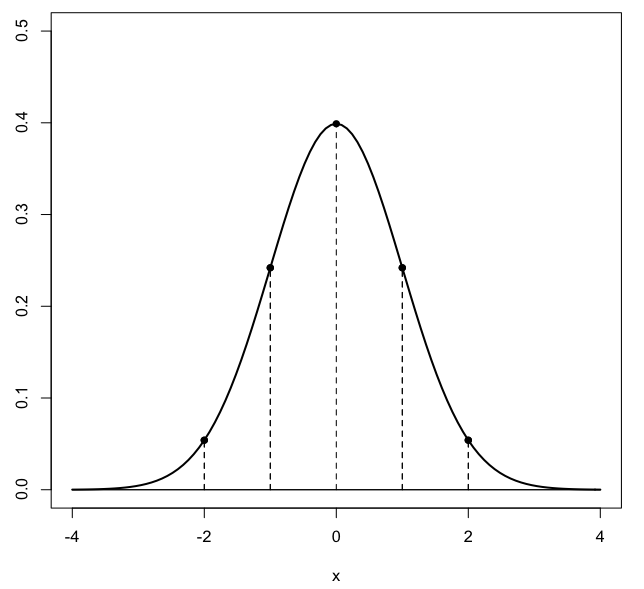
\includegraphics [scale=0.4] {gauss3.png} \end{center}
\begin{document}
\maketitle
\Large
Here we look at some properties of the set $\mathbb{R}$ of real numbers.  The standard sets also include $\mathbb{N}$, the natural or counting numbers $\{1,2,3, \dots\}$, also known as the positive integers, and the complete set of integers $\mathbb{Z} = \{0, \pm \ 1, \pm \ 2, \dots\}$.

A particular interest is similarities and differences between $\mathbb{R}$ and another one of its subsets, the set $\mathbb{Q}$ of rational numbers.  Q likely stands for quotient as in the notation $p/q$ (for $p \in \mathbb{Z}$ and $q \in \mathbb{N}$).

An important property of the rational numbers is that no matter how close two such numbers are, we can always construct another rational number that lies between them (by simply averaging).  

And yet, there are "holes" in the number line constructed from $\mathbb{Q}$.  There is a hole at $n=\sqrt{2}$, which cannot be expressed as a rational number, and another one at $e$, and still others at $\sqrt{3}$, $\pi$ and so on.

In fact, Cantor showed that the density of the real numbers is much much greater than that of the rationals.  One analogy is that rational numbers are like stars and real numbers like the space between them (or maybe dark matter or something).

Enough with the analogies.  Let's start with some definitions:

$\bullet$  A \emph{sequence} ($a_n$) can be considered to be a \emph{function} from the natural numbers $\mathbb{N}$ to $\mathbb{R}$ (written as $f: \mathbb{N} \rightarrow \mathbb{R}$).  The elements or members of a sequence are written with subscripts, usually starting with $a_1$:
\[ (a_n) = a_1, a_2, \dots a_n, \dots\]
which may just be written as
\[ a_1, a_2, \dots a_n, \]

A sequence does not terminate, it has an infinite number of terms.  We are usually most interested in the long-term behavior of a sequence, and may disregard what happens for $a_n$ where $n > N$, for some fixed $N$.

$\bullet$  A sequence ($a_n$) is called \emph{increasing}
\[ \iff a_{n+1} \ge a_n \]

We use the symbol $\iff$ to mean \emph{if and only if}.

Although we might have written $\forall \ n \in \mathbb{N}$ (for every $n$ in the set $\mathbb{N}$ of natural numbers) to preface the statement above, we will leave that as understood.

$\bullet$  It is \emph{not} necessary for each term in an increasing sequence to be strictly larger than the previous one as long as $a_{n+1} \ge a_n$.

$\bullet$  If $a_{n+1} > a_n$ always, the sequence is \emph{strictly increasing}.

$\bullet$  An increasing sequence may be \emph{monotonic} $\iff$ it is \emph{non-decreasing}.  Just as with an increasing sequence, a monotonic sequence does not have to be strictly increasing.  If the terms do not change at all, it still qualifies as monotonic.

I would divide monotonic sequences into three cases:  (i) all terms the same, (ii) terms strictly increasing, with $a_{n+1} > a_n$ always, and (iii) sometimes $a_{n+1} > a_n$ and sometimes $a_{n+1} = a_n$.  

I claim that we can convert case (iii) into case (ii) by dropping every $a_{n}$ for which $a_n = a_{n-1}$, focusing on the behavior of the strictly increasing version.

$\bullet$  Similar definitions can be given for a \emph{decreasing} sequence.  The steps in the theory we will sketch can be equally applied to decreasing sequences, but we will focus on the case of increasing ones.

$\bullet$  The set $\mathbf{X}$ is \emph{bounded above}
\[\iff \exists \ M \in \mathbb{R} \ | \ \forall \ x \in X, x \le M\]
$\mathbf{X}$ is bounded above if we can find a real number $M$ which is greater than or equal to all the members of the set.

$\bullet$  Similarly, the sequence ($a_n$) is \emph{bounded above} if and only if we can find a real number $M$ which is greater than or equal to all the terms in the sequence.

\subsection*{epsilon-delta}
Formal proofs in analysis typically use small numbers termed $\epsilon$ and $\delta$.  We introduce the method in the context of finding a limit $L$ to a function $f(x)$ as $x \rightarrow c$, where $c$ is some real number.

We say that, \emph{if} for all points $x$ within a specified distance $\delta$ of $c$
\[  0 < | x - c| < \delta \]
we find that $f(x)$ lies within a specified distance $\epsilon$ from $L$
\[ |f(x) - L| < \epsilon \]
\emph{then} the limit is $L$.

To do this, $\epsilon$ is chosen first.  For that reason I call it a game.  Why don't you go first?  

$\epsilon$ provides a constraint on how close to $L$ you want the value of $f(x)$ to be.  However I insist that you choose $\epsilon \ne 0$;  we do not require that $c$ even be within the domain of $f$.

We then require that the \emph{difference} between $f(x)$ and $L$ must be less than $\epsilon$.

I try to find a suitable $\delta$ to make this be true.  If I can find such a $\delta$, then you get another chance, and will presumably choose a smaller $\epsilon$.  

If I can prove that it is possible to find a $\delta$ to guarantee that your constraint is satisfied for \emph{all} values of $\epsilon > 0$ \emph{no matter how small}, then I win and the limit exists.  If not, it doesn't.

\subsection*{simple example}
Suppose $f(x) = 2x$ and I claim that the limit $L$ as $x \rightarrow 1$ is equal to $2$.  You choose any $\epsilon > 0$, then I choose $\delta < \epsilon/2$.  As long as $|1 - x| < \epsilon/2$, the absolute value $|L - f(x)| < \epsilon$. 

\subsection*{definition}
Here is a formal definition:
\[ \forall \ \epsilon > 0, \exists \ \delta > 0 \ | \ \forall \ x, \ 0 < | x - c| < \delta \rightarrow | f(x) - L | < \epsilon \]

$\circ$  for \emph{any} real number epsilon $\epsilon > 0$

$\circ$  there exists (we can find) a real number delta $\delta > 0$ 

$\circ$  such that for all $x$

$\circ$  if c - $\delta < x  < c + \delta$ (equivalent to $ | x - c| < \delta$)

$\circ$  then $f(x) - \epsilon < L  < f(x) + \epsilon$

\subsection*{back to sequences}
$\bullet$  Suppose that $(a_n)$ is a sequence and $L$ is a real number. If for all $\epsilon > 0$, we can find a term in the sequence such that it differs from $L$ by less than $\epsilon$ 
\[ |a_n - L | < \epsilon \]
and the same is true for all subsequent terms, then the sequence $(a_n)$ is \emph{convergent} and $L$ is its \emph{limit}.

We combine the previous concepts of a bounded monotone sequence and convergence:

\textbf{Axiom}  (Monotone Sequence Property). \emph{Any bounded monotone sequence converges.}

Beck:
\begin{quote}This axiom (or one of its many equivalent statements) gives arguably the most important property of the real number system; namely, that we can, in many cases, determine that a given sequence converges without knowing the value of the limit. In this sense we can use the sequence to define a real number.\end{quote}

Beck continues on to say that this property implies the next one:

$\bullet$ Any bounded monotone, and thus convergent, sequence has a \emph{least upper bound}.

\subsection*{supremum and infinum}
$\bullet$  In set theory, the \emph{supremum} of a subset $\mathbf{S}$ of a partially ordered set $\mathbf{T}$ is the least element in $\mathbf{T}$ that is greater than or equal to all elements of $\mathbf{S}$.

I think it's easier to see this with an example.  Suppose we define a set
\[ \mathbf{A} = x \in \mathbb{R} \ | \ \ 0 < \ x \le 5 \]
The set $\mathbf{A}$ includes the real number $5$, and $5$ is its largest element.  Every element $x$ in $\mathbf{A}$ is less than or equal to $5$.  $\mathbf{A}$ has a \emph{maximum element}.

On the other hand, suppose we had defined $\mathbf{B}$ as
\[ \mathbf{B} = x \in \mathbb{R} \ | \ \ 0 < \ x < 5 \]
This set does not include the real number $5$.  Furthermore, it isn't possible to specify a largest element in the latter case.  (If you pick one, then I can always find another real number larger than yours and closer to $5$ --- see below).  

We use a new word \emph{supremum} to describe the relationship of the number $5$ for these sets.  $5$ is the supremum for both $\mathbf{A}$ and $\mathbf{B}$.  The supremum of a set need not belong to the set.  If a set has a maximum element then that element is its supremum.

Supremum and \emph{least upper bound} mean the same thing.

In a similar fashion, $0$ is the \emph{infinum} for both sets.

\subsection*{infinity}

more to say here

\end{document}}